\documentclass{beamer}


\usepackage{a4wide}
\usepackage{amsmath}
\usepackage{amssymb}
\usepackage{amsthm}
\usepackage[czech]{babel}
\usepackage{bookmark}
\usepackage{enumerate}
\usepackage[T1]{fontenc}
\usepackage{forest}
\usepackage{hyperref}
\usepackage[utf8]{inputenc}
\usepackage{lmodern}
\usepackage{multicol}
\usepackage{tikz}

\theoremstyle{definition}
    \newtheorem{problem}{Příklad}

% \theoremstyle{remark}
%     \newtheorem*{steps}{Postup řešení}

\theoremstyle{plain}
    \newtheorem*{solution}{Řešení}
    

\DeclareRobustCommand\proves{\mathrel{|}\joinrel\mkern-.5mu\mathrel{-}}
\DeclareMathOperator{\Conseq}{Csq}
\DeclareMathOperator{\M}{M}

% hide solutions
\newif\ifhidesolutions
    \hidesolutionstrue
    % \hidesolutionsfalse

\ifhidesolutions
    \usepackage{environ}
    \NewEnviron{hide}{}
    \let\solution\hide
    \let\endsolution\endhide
\fi








\title{První přednáška}
\subtitle{NAIL062 Výroková a predikátová logika}
\author{Jakub Bulín (KTIML MFF UK)}
% \institute{KTIML MFF UK}
\date{Zimní semestr 2023}


\begin{document}


\frame{\titlepage}


\begin{frame}{Cesta k jistému úspěchu u zkoušky\footnote{Podrobnosti o zkoušce včas upřesníme. Základní formát i většina otázek ale pravděpodobně zůstanou stejné, viz loňské \href{https://jbulin.github.io/teaching/fall/nail062/files/info-o-zkouskach.pdf}{\alert{\textbf{informace o zkouškách}}}.}}

\begin{itemize}    
    \item Studujte \alert{průběžně (každý týden)}, a průběžně také \alert{testujte své znalosti}: umíte sami \alert{napsat}(!) definici, větu, důkaz?
    \item Před každou přednáškou alespoň zběžně projděte příslušné sekce v \href{https://github.com/jbulin-mff-uk/nail062/raw/main/lecture/lecture-notes/lecture-notes.pdf}{\alert{\textbf{Zápiscích z přednášky}}}. Ty obsahují vše, co po vás bude vyžadováno.\footnote{Nedoporučujeme učit se primárně podle slidů! Mnoho detailů v nich chybí.} Snažte se pochopit smysl definic a tvrzení.
    \item Po každé přednášce si skripta \alert{podrobně přečtěte}. Pokud něčemu nebudete rozumět, využijte konzultačních hodin.
    \item Snažte se zúčastnit všech přednášek, pokud nemůžete, včas se materiál doučte, případně využijte konzultačních hodin.
    \item Ujistěte se, že rozumíte nejen myšlenkám, ale umíte pracovat i s \alert{formalizmem}: ten je neoddělitelnou součástí logiky.
    \item Stejnou pozornost věnujte i přípravě na \alert{cvičení}.
    \bigskip
\end{itemize}

\end{frame}


\begin{frame}{První přednáška}

    \textbf{Program}
        \begin{itemize}
            \item úvod do logiky
            \item neformální představení výrokové a predikátové logiky
            \item syntaxe výrokové logiky
        \end{itemize}        


    \textbf{Materiály}

        \href{https://github.com/jbulin-mff-uk/nail062/raw/main/lecture/lecture-notes/lecture-notes.pdf}{\alert{\textbf{Zápisky z přednášky}}}, Kapitola 1 a Sekce 2.1 z Kapitoly 2


\end{frame}


\section{\sc Kapitola 1: Úvod do logiky}


\begin{frame}{Co je logika?}

    % 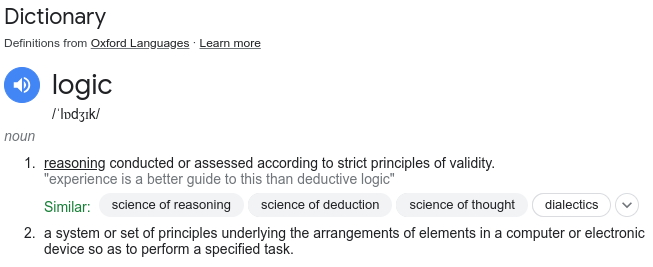
\includegraphics[width=\textwidth]{slides1-images/definiton-of-logic.png}
    
    \href{https://www.google.com/search?q=define+logic}{\textbf{Dvě definice:}}
        \begin{enumerate}
            \item soubor principů, které jsou základem uspořádání prvků nějakého systému (např.\ počítačového programu, elektronického zařízení, komunikačního protokolu)
            \item věda o uvažování prováděném podle striktních pravidel zachovávajících platnost 
        \end{enumerate}        


    \myblock{\textbf{V informatice obojí:} daný systém nejprve \emph{formálně popíšeme}, a poté o něm \emph{formálně uvažujeme} (automaticky!), tj. odvozujeme \alert{platné inference} za použití nějakého \alert{dokazovacího systému}
    }

\end{frame}


\begin{frame}{Historie a aplikace logiky}

    {\footnotesize Filozofie $\to$}  {\normalsize Matematika $\to$}  {\large Teoretická informatika $\to$} 
        
    \myalertinline{\Large Aplikovaná informatika}

    \begin{itemize}
        \item logic programming
        \item discrete optimization (SAT solving, scheduling, planning)
        \item database theory
        \item verification (software, hardware, protocol)
        \item automated reasoning and proving
        \item knowledge-based representation
        \item artificial intelligence
    \end{itemize}

\end{frame}


\section{1.1 Výroková logika}


\begin{frame}{Příklad ze života: Hledání pokladu}

    \myexample{
        Při hledání pokladu jsme narazili na rozcestí dvou chodeb. Víme, že na konci každé chodby je buď poklad, nebo drak, ale ne obojí. 
        
        \medskip
        Trpaslík nám řekl, že: 
        \begin{itemize}
            \item \emph{``Alespoň jedna z těch dvou chodeb vede k pokladu''}, a že
            \item \emph{``První chodba vede k drakovi.''}
        \end{itemize}

        \medskip
        Je známo, že trpaslíci buď vždy mluví pravdu, nebo vždy lžou. Kterou cestou se máme vydat?
    }

\end{frame}


\begin{frame}{Výroky neformálně}

    \alert{Výrok} je tvrzení, kterému lze přiřadit pravdivostní hodnotu: 
    \begin{center}
        \alert{pravdivý} (\emph{True}, 1), nebo \alert{lživý} (\emph{False}, 0)
    \end{center}
    
    \alert{Prvovýroky} (\alert{atomické výroky}, \alert{výrokové proměnné}) zkombinované pomocí logických spojek a závorek do \alert{složených výroků}:

    \myexample{
        ``(Trpaslík lže,) \emph{právě když} (druhá chodba vede k drakovi.)''\
    }        

    \begin{description}\setlength{\itemsep}{3pt}
        \item[\huge\alert{$\neg$}] ``neplatí X'', \emph{negace}
        \item[\huge\alert{$\landsymb$}] ``X a Y'', \emph{konjunkce}
        \item[\huge\alert{$\lorsymb$}] ``X nebo Y'', \emph{disjunkce} (není exkluzivní)
        \item[\huge\alert{$\limpliessymb$}] ``pokud X, potom Y'', \emph{implikace} (čistě logická)
        \item[\huge\alert{$\liffsymb$}] ``X, právě když Y'', \emph{ekvivalence}
    \end{description}

\end{frame}


\begin{frame}{Formalizace ve výrokové logice}

    Volba množiny prvovýroků: \myalertinline{bity informace popisující daný systém}
    
    \myexample{            
        $p_1=${\it ``Poklad je v první chodbě.''}\\
        $p_2=${\it ``Poklad je ve druhé chodbě.''}
    }\vspace{-12pt}

    (Co nejmenší, např. hodnota $t=${\it ``Trpaslík mluví pravdu.''} je jednoznačně určená hodnotami $\mathbb P=\{p_1,p_2\}$.)
    \begin{itemize}
        \item {\it Poklad nebo drak, ale ne obojí}: zakódované do volby $\mathbb P$ (přítomnost draka je absence pokladu)
        \item {\it ``První chodba vede k drakovi.''} $\Leftrightarrow$ \alert{$\neg p_1$}
        \item {\it ``Alespoň jedna z chodeb vede k pokladu.''} $\Leftrightarrow$ \alert{$p_1 \lor p_2$}
        \item {\it Trpaslík buď mluví pravdu, nebo lže}:
        \myexamplemath{
        $$
        \varphi = (\neg p_1 \land (p_1 \lor p_2)) \lor (\neg (\neg p_1) \land \neg (p_1 \lor p_2))
        $$
        }
    \end{itemize}

    \medskip
    \myblock{
    \alert{Teorie} $T=\{ \varphi \}$ v \alert{jazyce} $\mathbb P=\{p_1,p_2\}$, $\varphi$ je \alert{axiom} $T$.
    }

\end{frame}


\begin{frame}{Modely a důsledky}

    Lze určit, kde je poklad? Je $p_1$ nebo $p_2$ \alert{důsledkem} $\varphi$ resp. $T$?    

    \alert{``Svět''}, ve kterém je např. v první chodbě poklad a ve druhé drak, popíšeme pomocí \alert{pravdivostního ohodnocení} $p_1=1,p_2=0$, neboli \alert{modelu} $v=(1,0)$ jazyka $\mathbb P$. Celkem máme 4 ``světy'' a modely:
    \myexample{\vspace{-6pt}
    $$
    \M_\mathbb P=\{(0,0),(0,1),(1,0),(1,1)\}.
    $$
    }
    Je ``svět'' popsaný modelem $v = (1,0)$ \emph{konzistentní} s tím, co víme, tj. \alert{platí} v modelu $v$ výrok $\varphi$ resp. teorie $T$? Vyhodnotíme podle stromové struktury $\varphi$:
    $$
    v(p_1) = 1,\ v(p_2) = 0,\ v(\neg p_1) = 0,\ v(p_1 \lor p_2)=1,\ \dots,\ \alert{v(\varphi)=0}
    $$
    Množina \alert{modelů výroku} \( \varphi \) (resp.\ \emph{modelů teorie} \( T \)):
    \myexample{\vspace{-6pt}
    $$
    \M_\mathbb P(\varphi)=\M_\mathbb P(T)=\{(0,1)\}.
    $$
    }

    \vspace{-12pt}
    \myblock{V \alert{každém modelu} teorie $T$ platí výrok $p_2$, neboli $p_2$ je \alert{důsledek}~$T$.}
    
\end{frame}


\begin{frame}{Důkazové systémy}

    Ověřovat všechny modely je nepraktické, pro $|\mathbb P|=n$ máme $2^n$ modelů, a $\mathbb P$ může být i nekonečná.

    \textbf{Důkazový systém}
    \begin{itemize}
        \item \alert{důkaz} výroku~\( \psi \) z teorie \(T\) je formálně definovaný syntaktický objekt, snadno (mechanicky) ověřitelný
        \item lze hledat algoritmicky čistě na základě struktury \( \psi \) a axiomů \(T\) (``\emph{syntaxe}''), nemusíme se zabývat modely (``\emph{sémantikou}'').
    \end{itemize}        
    Klíčové vlastnosti:

    \myblock{
    \begin{itemize}
        \item \alert{korektnost}: pokud existuje důkaz \( \psi \) z \(T\), potom \( \psi \) platí v \(T\)
        \item \alert{úplnost}, pokud \( \psi \) platí v \(T\), potom existuje důkaz \( \psi \) z \(T\)
    \end{itemize}
    }

    %Korektnost je nutná, ale efektivní důkazový systém může být užitečný, i pokud v něm nelze dokázat vše, co platí.
    Ukážeme si \alert{metodu analytického tabla} a \alert{rezoluční metodu}. Obě dokazují \emph{sporem}: předpokládají platnost $T$ a \( \neg \psi \), hledají spor.

\end{frame}

%\section{tablo metoda (neformálně)}

\begin{frame}{Metoda analytického tabla}

\begin{itemize}
    \item důkaz je strom olabelovaný předpoklady o platnosti výroků
    \item v kořeni: \alert{neplatí} dokazovaný výrok $\psi$ (důkaz sporem)
    \item připojíme platnost axiomů z $T$
    \item dále budujeme tablo zjednodušováním výroků ve vrcholech, podle pravidel zaručujících následující \alert{invariant}:\medskip
    
    \myalert{
        Každý model teorie \(T\), ve kterém neplatí \(\psi\), se musí \emph{shodovat} s některou z větví tabla. 
    }
    
    \vspace{-6pt}
    \item například:\medskip
    \myblock{
    \alert{\small True $(\varphi_1 \limplies \varphi_2 )$} zredukujeme rozvětvením na \alert{\small False $\varphi_1$} a \alert{\small True $\varphi_2$},\\
    \alert{\small False $(\varphi_1 \limplies \varphi_2 )$} zredukujeme připojením \alert{\small True $\varphi_1$} a \alert{\small False $\varphi_2$}.
    }
        
    \vspace{-6pt}
    \item \alert{sporná} větev = předpokládá True i False stejného výroku
    \item \alert{důkaz} = všechny větve sporné (tj. nemůže existovat model $T$, ve kterém neplatí $\psi$)
\end{itemize}

\end{frame}


\begin{frame}{Příklad tablo důkazu}

    \vspace{-6pt}
    \begin{figure}\scalebox{0.8}{\small
        \centering
        \begin{forest}
        [False \( p_2 \)
            [True \( (\neg p_1 \land (p_1 \lor p_2)) \lor (\neg (\neg p_1) \land \neg (p_1 \lor p_2)) \) 
                [True \( \neg p_1 \land (p_1 \lor p_2) \)
                    [True \( \neg p_1 \)
                        [True \( p_1 \lor p_2 \)
                            [False \( p_1 \)
                                [True \( p_1 \), tikz={\node[fit to=tree,label=below:\alert{fail}] {};}
                                ]
                                [True \( p_2 \), tikz={\node[fit to=tree,label=below:\alert{fail}] {};}
                                ]
                            ]
                        ]
                    ]
                ]
                [True \( \neg (\neg p_1) \land \neg (p_1 \lor p_2) \)
                    [True \( \neg (\neg p_1) \)
                        [True \(\neg (p_1 \lor p_2) \)
                            [False \( (\neg p_1) \)
                                [True \( p_1 \)
                                    [False \(p_1 \lor p_2 \)
                                        [False \(p_1\)
                                            [False \(p_2\), tikz={\node[fit to=tree,label=below:\alert{fail}] {};}
                                            ]
                                        ]
                                    ]
                                ]
                            ]
                        ]
                    ]
                ]
            ]
        ]
        \end{forest}

    }
    \end{figure}    

\end{frame}


%\section{rezoluční metoda (neformálně)}


\begin{frame}{Konjunktivní normální forma (CNF)}

    \alert{literál} $p$, $\neg p$\hfill \alert{klauzule} disjunkce literálů\hfill \alert{CNF} konjunkce klauzulí

    \myblock{
        každý výrok má \alert{ekvivalentní} CNF (\alert{$\psi \sim \psi'$}, stejné modely)
    }

    
    \vspace{-12pt}
    \myexample{např. pro výrok 
    $
    (\neg p_1 \land (p_1 \lor p_2)) \lor (\neg (\neg p_1) \land \neg (p_1 \lor p_2))
    $
    }

    \vspace{-12pt}

    nahradíme \alert{$\neg (\neg p_1) \sim p_1$} a \alert{$\neg (p_1 \lor p_2) \sim (\neg p_1 \land \neg p_2)$} (\emph{De Morgan})

    \myexamplemath{
    $$
    (\neg p_1 \land (p_1 \lor p_2)) \lor (p_1 \land \neg p_1 \land \neg p_2)
    $$
    }

    \vspace{-18pt}

    a dále opakovaně použijeme \alert{distributivitu} \( \lorsymb \) vůči \( \landsymb \): \medskip

    \myexamplemath{\vspace{-12pt}
    \begin{gather*}
    (\neg p_1 \lor p_1) \land (\neg p_1 \lor \neg p_1) \land (\neg p_1 \lor \neg p_2) \land (p_1 \lor p_2 \lor p_1) \land\\ (p_1 \lor p_2 \lor \neg p_1)\land (p_1 \lor p_2 \lor \neg p_2)    
    \end{gather*}    
    }

    \vspace{-6pt}
    už je CNF, ještě zjednodušíme: odstraníme duplicitní literály, a klauzule obsahující $p_i$ a zároveň $\neg p_i$ (to jsou \alert{tautologie})

    \myexamplemath{
    $$
    \neg p_1 \land (\neg p_1 \lor \neg p_2) \land (p_1 \lor p_2)
    $$
    }
\end{frame}


\begin{frame}{Rezoluční důkaz}

Důkaz sporem: převedeme \alert{negaci} dokazovaného do CNF a přidáme

\myblock{
\alert{\(p_2\) platí v \(T\)}, právě když je následující CNF výrok \alert{nesplnitelný}:
}
\myexamplemath{
$$
\neg p_1 \land (\neg p_1 \lor \neg p_2) \land (p_1 \lor p_2)\land\alert{\neg p_2}
$$
}\vspace{-6pt}

množinový zápis:
\myexampleinline{$
S=\left \{ \{\neg p_1\},\{\neg p_1,\neg p_2\},\{p_1, p_2\},\{\neg p_2\} \right \}
$
}

\myalert{\alert{rezoluční pravidlo}: je-li $p\in C_1$ a $\neg p\in C_2$, potom \emph{rezolventa} 
$$
C= (C_1\setminus \{p\})\cup(C_2\setminus \{\neg p\})
$$ platí v každém modelu, ve kterém platí $C_1$ i $C_2$
}

\alert{rezoluční zamítnutí $S$}: posloupnost klauzulí, kde každá je buď z $S$ nebo rezolventa předchozích, poslední je prázdná klauzule $\square$

\myblock{protože $\square$ nemá žádný model, je i $S$ nesplnitelná}

\end{frame}


\begin{frame}{Příklad rezolučního důkazu}

\alert{rezoluční zamítnutí} (třetí klauzule je rezolventou 1. a 2., pátá je rezolventou 3. a 4.)
\myexample{\vspace{-6pt}
\[
    \{\neg p_1\},\{p_1, p_2\},\{p_2\},\{\neg p_2\},\square
\]
}


\alert{rezoluční strom} (listy klauzule z $S$, vnitřní vrcholy rezolventy synů) 
\myexample{
    \begin{center}
        \begin{forest}
        for tree={grow=north}
        [\( \square \)
            [\( \{\neg p_2\} \)]
            [\( \{p_2\} \)
            [{\( \{p_1, p_2\} \)}]
            [\( \{\neg p_1\} \)]
            ]
        ]
        \end{forest}
    \end{center}
}
\end{frame}



%\section{příklad: barvení grafů}


\begin{frame}{Příklad: Barvení grafů}

    \myexample{
    Najděte vrcholové obarvení následujícího grafu třemi barvami.
    \begin{center}
    \begin{tikzpicture}[every node/.style={circle,fill=blue!10,draw,minimum size=0.5cm,node distance=1.5cm}]
    \node (1) {$1$};
    \node[right of=1] (2) {$2$};
    \node[below of=2] (3) {$3$};
    \node[left of=3] (4) {$4$};
    \path[draw] (1) -- (2) -- (3) -- (4) -- (1) -- (3);
    \end{tikzpicture}
    \end{center}
    }

    
    graf: množina vrcholů a množina (libovolně) \alert{orientovaných} hran
    \[
    \mystructure G = \langle V; E \rangle = \langle \{1,2,3,4\}; \{(1,2),(1,3),(1,4),(2,3),(3,4)\} \rangle
    \]
    jak formalizovat? pro $v\in V$ a $c\in C=\{R,G,B\}$:
    \myalertmath{
    $$
    p_v^c=\text{\it``vrchol \(v\) má barvu \(c\)''}
    $$
    }

    \vspace{-12pt}

    \mbox{\small $\mathbb P=\{p_v^c\mid c\in C,v\in V\}=\{p_1^R,p_1^G,p_1^B,p_2^R,p_2^G,p_2^B,p_3^R,p_3^G,p_3^B,p_4^R,p_4^G,p_4^B\}$}

máme celkem \( |\M_\mathbb P|=2^{12}=4096 \) \alert{modelů jazyka} (12-dim. vektorů)
\end{frame}


\begin{frame}{Formalizace hranového obarvení}
\begin{itemize}
    \item každý vrchol má nejvýše jednu barvu: $4^4=2^8=256$ modelů

    \myexample{\vspace{-12pt}
    $$
    T_1 = \{ (\neg p_v^R \lor \neg p_v^G) \land (\neg p_v^R \lor \neg p_v^B) \land (\neg p_v^G \lor \neg p_v^B) \mid v \in V \}
    $$
    }
    \item a každý vrchol má alespoň jednu barvu: $3^4=81$ modelů
    
    \myexample{\vspace{-12pt}
    $$T_2 = T_1\cup \{ p_v^R \lor p_v^G \lor p_v^B \mid v \in V \}= T_1\cup \{\bigvee_{c\in C} p_v^c \mid v \in V \}
    $$
    }
    $T_2$ je \alert{extenze} teorie $T_1$ neboť \alert{každý důsledek $T_1$ platí i v $T_2$}, zde dokonce $\M_\mathbb P(T_2)\subseteq\M_\mathbb P(T_1)$
    %\footnote{Proč $\subseteq$? Čím více vlastností požadujeme, tím méně objektů je splňuje.}

    \item nakonec přidáme \alert{hranovou podmínku}:
     
    \myexample{
    $$
    T_3 = T_2\cup \{ \bigwedge_{c\in C} 
    (\neg p_u^c \lor \neg p_v^c) \mid (u,v) \in E \}
    $$
    }  
    Výsledná teorie \( T_3 \) je \alert{splnitelná} (má model), právě když je graf \( \mystructure{G} \) 3-obarvitelný.   
\end{itemize}
\end{frame}


\begin{frame}{Co s ní?}

\textbf{Všechna obarvení?} 

$T_3$ má 6 modelů: \( v = (1,0,0,0,1,0,0,0,1,0,1,0) \) a další získané permutací barev \vspace{-12pt}
\begin{center}
    \begin{tikzpicture}[every node/.style={circle,fill=blue!10,draw,minimum size=0.3cm,node distance=1cm}]
    \node[fill=red] (1) {$1$};
    \node[fill=green,right of=1] (2) {$2$};
    \node[fill=blue,below of=2] (3) {$3$};
    \node[fill=green,left of=3] (4) {$4$};
    \path[draw] (1) -- (2) -- (3) -- (4) -- (1) -- (3);
    \end{tikzpicture}
\end{center}

\textbf{Obarvení, ve kterých je vrchol 1 modrý a vrchol 2 zelený?} 

Odpovídají modelům teorie \( T_3 \cup \{ p_1^B, p_2^G\} \)

\textbf{Důkaz, že vrcholy 2 a 4 musí mít stejnou barvu?}

\alert{Tablo} s kořenem $\text{False  }(p_2^R \land p_4^R)\lor(p_2^G \land p_4^G)\lor(p_2^B \land p_4^B)$

Nebo \alert{rezolucí}: přidáme \alert{negaci} \( (p_2^R \land p_4^R)\lor(p_2^G \land p_4^G)\lor(p_2^B \land p_4^B) \), vše převedeme do CNF a zamítneme

\end{frame}


\section{1.2 Predikátová logika}


\begin{frame}{Nevýhody formalizace ve výrokové logice}
Teorie $T_3$ je poměrně velká, a `natvrdo' kóduje graf $\mystructure G$.  

\begin{center}
    \begin{tikzpicture}[every node/.style={circle,fill=blue!10,draw,minimum size=0.5cm,node distance=1.5cm}]
    \node (1) {$1$};
    \node[right of=1] (2) {$2$};
    \node[below of=2] (3) {$3$};
    \node[left of=3] (4) {$4$};
    \path[draw] (1) -- (2) -- (3) -- (4) -- (1) -- (3);
    \node[right of=3] (5) {$5$};
    \path[draw] (2) -- (5) -- (3);
    \end{tikzpicture}
\end{center}
Obohatit jazyk $\mathbb P'=\mathbb P \cup \{ p_5^R,p_5^G,p_5^B\}
$ a vytvořit ještě větší teorii~$T'_3$ přidáním axiomů o vrcholu 5 a hranách $(2, 5), (3,5)$?

A co vlastnosti obecně platné o všech nebo mnoha grafech?

\myblock{
V \alert{predikátové logice} můžeme mluvit \alert{o vrcholech} pomocí \alert{proměnných} a přirozeně vyjádřit vlastnosti jako:
\begin{itemize}
    \item \emph{``z vrcholu \(u\) vede hrana do vrcholu \(v\)''}
    \item \emph{``vrchol \(u\) je zelený''}
\end{itemize}
}
\end{frame}


\begin{frame}{Predikátová logika: struktury a jazyk}

    \textbf{Modely} už nejsou 0--1 vektory, ale \alert{struktury}, např. naše (orientované) grafy: 
    \myexample{\vspace{-12pt}\scriptsize
    \begin{align*}
        &\mystructure G = \langle V^\mystructure G; E^\mystructure G \rangle = \langle \{1,2,3,4\}; \{(1,2),(1,3),(1,4),(2,3),(3,4)\} \rangle \\ 
        &\mystructure{G}' = \langle V^{\mystructure{G}'}; E^{\mystructure{G}'} \rangle = \langle \{1,2,3,4,5\}; \{(1,2),(1,3),(1,4),(2,3),(3,4),(2,5),(3,5)\} \rangle
    \end{align*}
    }\vspace{-6pt}
    \begin{itemize}
        \item množina vrcholů, a binární relace na této množině
        \item \alert{jazyk} specifikuje kolik \alert{relací} jakých arit má struktura mít, a symboly pro ně
        \item např. \alert{jazyk grafů} \( \mathcal L=\langle E \rangle \) (kde \(E\) je binární relační symbol)
        \item $\mystructure G$ a $\mystructure G'$ jsou \alert{struktury v jazyce} $\mathcal L$ (\alert{$\mathcal L$-struktury})   
        \item můžeme mít také \alert{funkce} a \alert{konstanty}, a symbol \alert{$=$} pro \alert{rovnost} 
    \end{itemize}

\end{frame}


\begin{frame}{Predikátová logika: syntaxe a sémantika}

    \textbf{Syntaxe}: místo prvovýroků \alert{atomické formule}, např. $E(x,y)$, kde $x,y$ jsou \alert{proměnné} reprezentující vrcholy; stejné logické spojky, ale navíc \alert{kvantifikátory}:
  
    \begin{description}
        \item[\alert{\( (\forall x) \)}] {\it``pro všechny vrcholy \(x\)''}
        \item[\alert{\( (\exists y) \)}] {\it``existuje vrchol \(y\)''}
    \end{description}
    (hrají roli ``konjunkce'' a ``disjunkce'' přes všechny prvky)
    
    \myexample{
    \begin{itemize}
        \item ``V grafu nejsou smyčky'': \alert{$(\forall x)(\neg E(x,x))$}
        \item ``Existuje vrchol výstupního stupně 1'': 
        \alert{$(\exists x)(\exists y)(E(x,y) \land (\forall z)(E(x,z) \limplies y=z))$}
    \end{itemize}    
    }

    \textbf{Sémantika}: V daném grafu \(\mystructure{G}\) a při \alert{dosazení} vrcholu \(u\) za proměnnou \(x\) a vrcholu \(v\) za proměnnou \(y\) \alert{vyhodnotíme} \( E(x,y) \) jako \alert{True}, právě když \alert{\( (u,v)\in E^{\mystructure{G}} \)}.
        
\end{frame}


\begin{frame}{Barvení grafů v predikátové logice}
      
Jazyk \alert{\( \mathcal L' =\langle E, R, G, B \rangle \)}, kde \(E\) je binární a \(R,G,B\) jsou unární relační symboly (\(R(x)\) znamená {\it``vrchol \(x\) je červený''}) 

$\mathcal L'$-struktura: graf s trojicí množin vrcholů

\vspace{-32pt}
\begin{flushright}
    \scalebox{0.75}{
        \tikz[every node/.style={circle,fill=blue!10,draw,minimum size=0.3cm,node distance=1cm}]{
        \node[fill=red] (1) {$1$};
        \node[fill=green,right of=1] (2) {$2$};
        \node[fill=blue,below of=2] (3) {$3$};
        \node[fill=green,left of=3] (4) {$4$};
        \path[draw] (1) -- (2) -- (3) -- (4) -- (1) -- (3);
        }
    }
\end{flushright}

\myexample{\vspace{-15pt}\small
\begin{align*}
\mystructure G_C &= \langle V^{\mystructure G_C}; E^{\mystructure G_C}, R^{\mystructure G_C}, G^{\mystructure G_C}, B^{\mystructure G_C} \rangle \\
&= \langle \{1,2,3,4\}; \{(1,2),(1,3),(1,4),(2,3),(3,4)\}, \{1\}, \{2,4\}, \{3\} \rangle    
\end{align*}
}

\( \mystructure{G}_C \) je \alert{expanze} \(\mathcal L\)-struktury \( \mystructure{G} \) \alert{do jazyka} \( \mathcal L' \).

\myexample{Nejvýše jedna barva, alespoň jedna barva, hranová podmínka:

\small
\begin{itemize}
    \item $(\forall x)((\neg R(x) \lor \neg G(x)) \land (\neg R(x) \lor \neg B(x)) \land (\neg G(x) \lor \neg B(x)))$
    \item $(\forall x)(R(x) \lor G(x) \lor B(x))$
    \item $(\forall x)(\forall y)(E(x,y) \limplies ((\neg R(x) \lor \neg R(y)) \land (\neg G(x) \lor \neg G(y)) \land (\neg B(x) \lor \neg B(y))))$
\end{itemize}
}

\end{frame}


\section{1.3 Další druhy logických systémů}


\begin{frame}{Predikátové logiky vyšších řádů}

    \begin{itemize}
        \item Predikátová logika, kde proměnné reprezentují jednotlivé vrcholy, je logika \alert{prvního řádu} (\alert{first-order}, \alert{FO})
        \item Logika \alert{druhého řádu} (\alert{second-order}, \alert{SO}): proměnné i pro množiny vrcholů a $n$-tic vrcholů (tj. relace, funkce)
        \smallskip

        \myexample{\it
            ``Každá neprázdná zdola omezená podmnožina má infimum.''
            {\small
            \begin{align*}
            &(\forall S)((\exists x)S(x) \land (\exists x)(\forall y)(S(y) \limplies x\leq y) \limplies  {}\\ 
            &(\exists x)((\forall y)(S(y) \limplies x\leq y) \land (\forall z)((\forall y)(S(y) \limplies z\leq y)\limplies z\leq x)))
            \end{align*}
            }
        }
        \item A v logice \emph{třetího řádu} máme i množiny množin (např. v topologii).
    \end{itemize}

\end{frame}


\begin{frame}{Logiky zobecňující pojem pravdy}
    Kromě toho lze zobecnit pojem platnosti (pravdy):
    
    \begin{itemize}        
        \item \alert{temporální logiky} (platnost `vždy', `někdy v budoucnosti', `dokud' apod.) -- např. v paralelním programování
        \item \alert{modální logiky} (`je možné', `je nutné') -- v umělé inteligenci, uvažování autonomních agentů o svém okolí
        \item \alert{fuzzy logiky} (`je 0.35 pravdivé') -- v automatických pračkách
        \item \alert{intuicionistická logika} (povoluje jen konstruktivní důkazy, nemá \emph{zákon vyloučeného třetího})
    \end{itemize}
\end{frame}


\section{1.4 O přednášce}


\begin{frame}{Obsah předmětu}

    \begin{enumerate}[I.]
        \item Výroková logika (5 přednášek)
        \begin{itemize}
            \item Syntaxe a sémantika
            \item Problém SAT
            \item Tablo metoda
            \item Rezoluční metoda
        \end{itemize}
        \item Predikátová logika (6 přednášek)
        \begin{itemize}
            \item Syntaxe a sémantika
            \item Tablo metoda v predikátové logice
            \item Rezoluční metoda v predikátové logice
            \item Aplikace: databáze, Prolog, verifikace
        \end{itemize}
        \item Pokročilé partie (2 přednášky)
        \begin{itemize}
            \item Teorie modelů
            \item Nerozhodnutelnost a neúplnost
        \end{itemize}
    \end{enumerate}    

\end{frame}


\section*{ČÁST I -- VÝROKOVÁ LOGIKA}


\section{\sc Kapitola 2: Syntaxe a sémantika výrokové logiky}


\begin{frame}{Syntaxe a sémantika}
    \alert{syntaxe} dává pravidla pro tvoření korektních formálních výrazů sestávajících ze symbolů, a pro operace s nimi (\emph{výrok}, \emph{důkaz}, \dots)
    
    \alert{sémantika} popisuje význam syntaktických objektů ``v reálném světě'' (\emph{model}, \dots)
        
    Klíčem k logice je \alert{vztah mezi syntaxí a sémantikou}:
    \begin{itemize}
        \item sémantické objekty studujeme pomocí syntaxe (`jaké výroky platí v modelu?')
        \item syntaktické pomocí sémantiky, např. ekvivalence výroků: $\psi \sim \psi'$ právě když $\M_\mathbb P(\psi)=\M_\mathbb P(\psi')$
    \end{itemize}
\end{frame}


\section{2.1 Syntaxe výrokové logiky}


\begin{frame}{Jazyk}
    určený množinou \alert{prvovýroků} (\alert{výrokových proměnných}, \alert{atomických výroků}) -- neprázdná, konečná nebo i \emph{nekonečná}
    \myexample{\vspace{-18pt}
        \begin{align*}
            \mathbb P_1 &= \{ p, q, r\}\\
            \mathbb P_2 &= \{ p_0, p_1, p_2, p_3, \ldots \} = \{ p_i \mid i \in \mathbb N \}
        \end{align*}
    }
    (obvykle \emph{spočetná}, \emph{uspořádaná})

    dále do jazyka patří \alert{logické symboly}:
    \begin{itemize}
        \item logické spojky $\neg,\landsymb,\lorsymb, \limpliessymb, \liffsymb$
        \item závorky $(,)$
    \end{itemize}
\end{frame}


\begin{frame}{Výrok}

    \myblock{    
    \alert{Výrok} (\alert{výroková formule}) v jazyce $\mathbb P$ je prvek množiny $\VF_\mathbb P$ definované \emph{induktivně}: $\VF_\mathbb P$ je nejmenší množina splňující
    \begin{itemize}
        \item pro každý prvovýrok $p\in\mathbb P$ platí $p\in\VF_\mathbb P$,
        \item pro každý výrok $\varphi\in\VF_\mathbb P$ je $(\neg\varphi)$ také prvek $\VF_\mathbb P$
        \item pro každé $\varphi,\psi\in\VF_\mathbb P$ jsou $(\varphi\land\psi)$, $(\varphi\lor\psi)$, $(\varphi\limplies\psi)$, a $(\varphi\liff\psi)$ také prvky $\VF_\mathbb P$.
    \end{itemize}
    }

    \myalert{Výroky jsou nutně \emph{konečné} řetězce!}\vspace{-6pt}
    \alert{$\Var(\varphi)$}: množina všech prvovýroků ve $\varphi$ (vždy konečná)

    \alert{podvýrok}: podřetězec, který je sám výrok
    

    \myexample{
        $\varphi = ((p\lor (\neg q)) \liff (r\limplies (p \land q)))$, $\Var(\varphi)=\{p,q\}$\\
        podvýroky: $p, q, (\neg q), (p\lor (\neg q)), r, (p\land q), (r\limplies (p \land q)), \varphi$
    }\vspace{-6pt}
    
    \alert{pravda}: $\top=(p\lor(\neg p))$ , \alert{spor}: $\bot=(p\land(\neg p))$ \\
    (kde $p\in\mathbb P$ je pevně daný)

\end{frame}


\begin{frame}{Konvence zápisu}
    při \emph{zápisu} výroků můžeme vynechat některé závorky:
    \myexample{$\varphi = ((p\lor (\neg q)) \liff (r\limplies (p \land q)))$ lze zapsat jako $p\lor \neg q \liff (r\limplies p \land q)$}\vspace{-12pt}
    \begin{itemize}
        \item priorita operátorů: $\neg$ nejvyšší, dále $\landsymb$ a $\lorsymb$, nakonec $\limpliessymb$ a $\liffsymb$
        \item asociativita $\landsymb$ a $\lorsymb$: nápis $p\land q\land r$ znamená výrok $(p\land (q\land r))$
        \item vnější závorky nemusíme psát
    \end{itemize}

    \textbf{Poznámka:} v definici jsme mohli místo \emph{infixového} zápisu zvolit \emph{prefixový} (``polskou notaci''):
    {\it ``každý prvovýrok je výrok, jsou-li $\varphi,\psi$ výroky, jsou výroky také $\neg \varphi$, $\landsymb \varphi \psi$, $\lorsymb \varphi \psi$, $\limpliessymb \varphi \psi$, a $\liffsymb \varphi \psi$''} nebo i \emph{postfixový}
    
    \myexample{
        $\varphi=\liffsymb \lorsymb p \neg q \limpliessymb r \landsymb p q$\\
        $\varphi=p q \neg \lorsymb r p q \landsymb \limpliessymb \liffsymb$
    }

    \myalert{Důležitá je jen \alert{stromová struktura} výroků!}

\end{frame}


\begin{frame}{Strom výroku}   

    \myblock{
    \alert{$\Tree(\varphi)$} je zakořeněný uspořádaný strom, definovaný induktivně: 
        \begin{itemize}
            \item $\varphi=p\in\mathbb P$: jediný vrchol, s labelem $p$
            \item $\varphi=(\neg \varphi')$: kořen s labelem $\neg$, jediný syn je kořen $\Tree(\varphi')$.
            \item $\varphi=(\varphi' \lbin \varphi'')$ pro $\lbinsymb\in\{\landsymb,\lorsymb,\limpliessymb,\liffsymb\}$: kořen s labelem $\lbinsymb$ a dvěma syny: levý syn je kořen $\Tree(\varphi')$, pravý $\Tree(\varphi'')$.
        \end{itemize}
    }

    \bigskip

    \begin{columns}
        \column{0.55\textwidth}
        
        \myexample{$\varphi=((p\lor (\neg q)) \liff (r\limplies (p \land q)))$} 
            
        rekonstrukce $\varphi$ průchodem stromu, 
        podvýroky odpovídají podstromům

        \bigskip
        \myalert{$\Tree(\varphi)$ je jednoznačně určený!}

        \column{0.45\textwidth}
        \scalebox{0.9}{    
            \begin{forest}
                for tree={circle,draw=blue!20,fill=blue!10,minimum size=24pt}
                [$\liffsymb$ [$\lorsymb$ [$p$] [$\neg$ [$q$]]] [$\limpliessymb$ [$r$] [$\landsymb$ [$p$] [$q$]]]]
            \end{forest}
        } 
    \end{columns}

\end{frame}


\begin{frame}{Teorie}
    \myblock{
        \alert{Teorie} v jazyce $\mathbb P$ je libovolná množina výroků $T\subseteq\VF_\mathbb P$. Výrokům $\varphi\in T$ říkáme také \alert{axiomy}.
    }

    \myexample{
        $T=\emptyset$ a $T=\VF_\mathbb P$ nad libovolným jazykem,\\
        $T=\{p\land q,q\limplies (p\lor r)\}$ v jazyce $\mathbb P=\{p,q,r\}$\\
        $T=\{p_0\}\cup\{p_i\limplies p_{i+1}\mid i\in\mathbb N\}$ nad \emph{nekonečným} $\mathbb P=\{p_i\mid i\in\mathbb N\}$
    }

    \textbf{Poznámka:} \emph{Konečnou} teorii by bylo možné (byť ne praktické!) nahradit jediným výrokem: konjunkcí všech axiomů.
    
    Připouštíme ale i \emph{nekonečné teorie}; hodí se např. pro popis systému v (diskrétním) čase $t=0,1,2,\dots$.

\end{frame}


\end{document}
